\section{Appendix}

\section*{Amino acids}
\begin{table}[h]
\caption{Amino acids}
\centering
\begin{tabular}{l|l}
Letter	& Amino Acid	\\ \hline
A		& Alanine		\\
C		& Cysteine		\\
D		& Aspartic Acid	\\
E		& Glutamic Acid	\\
F		& Phenylalanine	\\
G		& Glycine		\\
H		& Histidine		\\
I		& Isoleucine	\\
K		& Lysine		\\
L		& Leucine		\\
M		& Methionine	\\
N		& Asparagine	\\
P		& Proline		\\
Q		& Glutamine		\\
R		& Arginine		\\
S		& Serine		\\
T		& Threonine		\\
V		& Valine		\\
W		& Tryptophan	\\
Y		& Tyrosine		\\

\end{tabular}
\end{table}

\section*{Secondary structures}

\begin{table}[H]
\caption{Q8 structure overview}
\centering
\begin{tabular}{l|l}
\hline 
Letter	& Secondary Structure 			\\ \hline
H	& Alpha-helix						\\
B	& residue in isolated beta bridge	\\
E	& extended strand					\\
G	& 3-helix							\\
I	& 5-helix							\\
T	& hydrogen bonded turn				\\
S	& bend								\\
L	& loop								\\
\end{tabular}
\end{table}

\begin{table}[H]
\caption{Q3 structure overview}
\centering
\begin{tabular}{l|l}
\hline
Letter		& Q8 structures in group	\\ \hline
H			& H, G						\\
B			& B, E						\\
C (coil)	& I, S, T, L				\\
\end{tabular}
\end{table}

\section*{Batch sizes}
A comparison of acheived accuracies on the validation and test set respectively performed on the unoptimized multi-task model can be seen below.
\begin{table}[H]
\centering
\begin{tabular}{lllllll}
\multicolumn{7}{c}{Layer debth = 80, kernel size = 11, learning rate = 0.00025, 3 hidden layers}                                                                                                                                                                                                                                                                                   \\ \hline
           & \multicolumn{3}{c|}{Validation set}                                                                                                                                                               & \multicolumn{3}{c}{Test set}                                                                                                                                      \\ \hline
Batch size & Q8 & \begin{tabular}[c]{@{}l@{}}Relative\\solvent\\accessibility\end{tabular} & \multicolumn{1}{l|}{\begin{tabular}[c]{@{}l@{}}Absolute\\solvent\\accessibility\end{tabular}} & Q8 & \begin{tabular}[c]{@{}l@{}}Relative\\ solvent\\ accessibility\end{tabular} & \begin{tabular}[c]{@{}l@{}}Absolute\\ solvent\\accessibility\end{tabular} \\ \hline
1          & 71.25\%     & 82.98\%                                                                       & \multicolumn{1}{l|}{81.41\%}                                                                       & 70.973\%    & 82.184\%                                                                   & 80.572\%                                                                \\
2          & 71.25\%     & 82.76\%                                                                       & \multicolumn{1}{l|}{81.21\%}                                                                       & 70.951\%    & 82.523\%                                                                   & 80.847\%                                                                \\
4          & 70.25\%     & 82.28\%                                                                       & \multicolumn{1}{l|}{80.84\%}                                                                       & 70.438\%    & 82.103\%                                                                   & 80.570\%                                                                \\
8          & 69.42\%     & 82.51\%                                                                       & \multicolumn{1}{l|}{80.73\%}                                                                       & 69.557\%    & 82.012\%                                                                   & 80.319\%                                                                \\
16         & 68.15\%     & 82.15\%                                                                       & \multicolumn{1}{l|}{80.42\%}                                                                       & 68.459\%    & 81.595\%                                                                   & 79.924\%                                                                \\
32         & 66.94\%     & 81.61\%                                                                       & \multicolumn{1}{l|}{79.85\%}                                                                       & 67.279\%    & 81.196\%                                                                   & 79.483\%                                                                \\
64         & 65.10\%     & 80.97\%                                                                       & \multicolumn{1}{l|}{79.25\%}                                                                       & 65.100\%    & 80.644\%                                                                   & 78.899\%                                                               
\end{tabular}
\end{table}

\section*{Layer depth}

\begin{figure}[H]
  \centering
  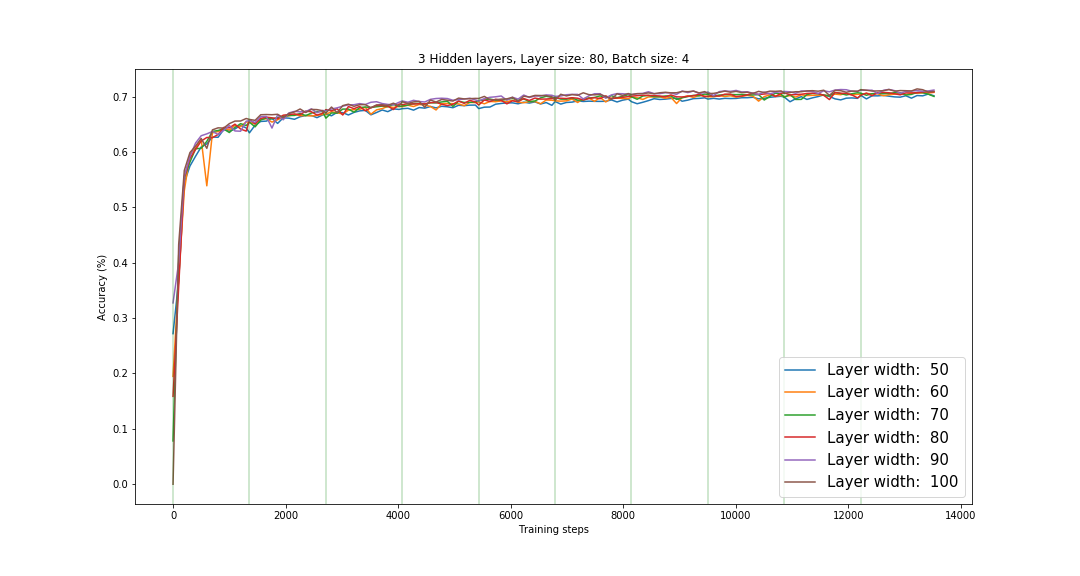
\includegraphics[width=\linewidth]{../graphs/new/layer_width_2}
  \caption{Accuracy on the validation set with varying layer depth.}
\end{figure}

\section*{Kernel sizes}

\begin{figure}[H]
  \centering
  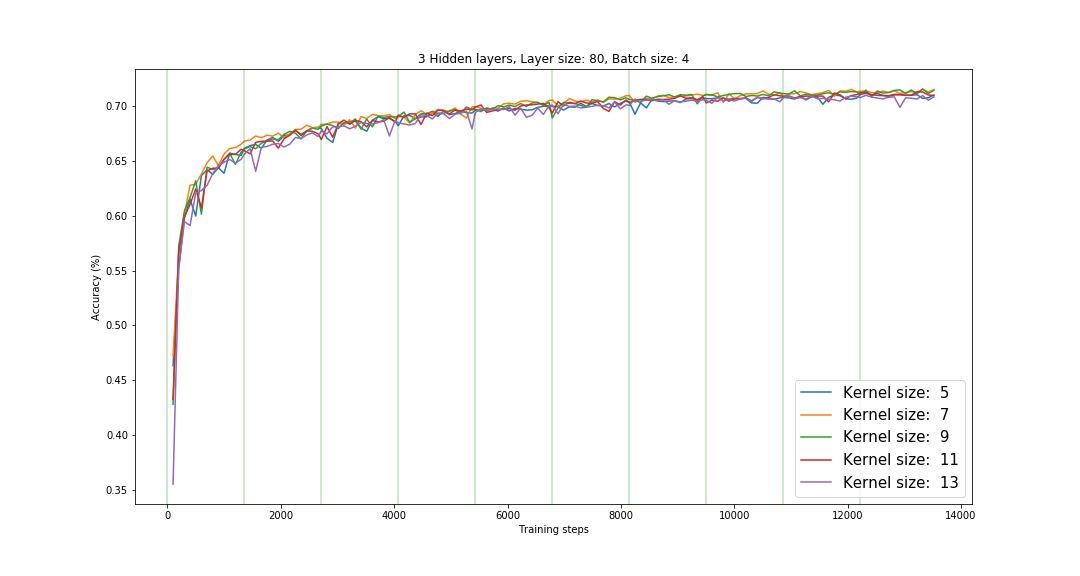
\includegraphics[width=\linewidth]{../graphs/new/kernel_size_1}
  \caption{All of the tested values for constant kernel size.}
\end{figure}